\documentclass[10pt,a4paper]{article}
\usepackage[T1]{fontenc}
\usepackage[utf8]{inputenc}
\usepackage{lmodern,microtype}
\usepackage[a4paper,left=1.75cm,right=1.75cm,top=1.55cm,bottom=1.55cm]{geometry}
\usepackage{amsmath,amssymb,xcolor,enumitem,setspace,graphicx}
\usepackage{titlesec}
\usepackage[hidelinks]{hyperref}
\usepackage{tikz}
\usetikzlibrary{positioning,arrows.meta,calc,fit}
\definecolor{titleblue}{HTML}{005293}
\definecolor{co2blue}{HTML}{2C7FB8}
\definecolor{poreblue}{HTML}{70B7DD}
\definecolor{zeogray}{HTML}{D9D3C7}
\definecolor{modelgreen}{HTML}{4C956C}
\setlength{\parindent}{1.2em}
\setlength{\parskip}{0pt}
\setlength{\emergencystretch}{2em}
\setstretch{1.0}
\setlist{itemsep=0.5pt,topsep=2pt,leftmargin=1.55em}
\titlespacing*{\section}{0pt}{1.4ex}{0.6ex}
\titlespacing*{\paragraph}{0pt}{1.2ex}{0.8em}
\pagestyle{empty}

\begin{document}
\begin{center}
{\Large\bfseries\color{titleblue}PoreAccess-CO$_2$:\par
From Random Packed-Bed Structure to a Fast Adsorption Model\par}
\vspace{0.55em}
{\normalsize Research concept proposal\par}
\vspace{0.2em}
{\small Ali Khalifa and Heiko Briesen\par
Technical University of Munich, Chair of Process Systems Engineering\par}
\end{center}
\vspace{0.25em}

\begin{abstract}
Packed beds are used for CO$_2$ adsorption, gas purification and drying. Even
when two beds contain the same monodisperse beads and have nearly the same porosity,
their void pathways can differ. These differences may control how easily gas
enters the bed and reaches the adsorbent, but they are hidden in conventional
one-dimensional models. This project will connect three model levels. DEM will
generate mechanically realistic zeolite beds. A pore-network model will resolve
diffusion and adsorption in each void structure. A simple homogeneous model
will then reproduce each uptake curve using one fitted effective diffusivity.
The central test is whether a physically defined inlet-accessibility descriptor
can predict this diffusivity for a new packing. The expected outcome is an
interpretable structure-to-model closure: particle geometry in, fast transient
adsorption prediction out. The study deliberately isolates diffusion-driven
adsorption; no CFD or imposed gas flow is required in the first step.
\end{abstract}

\section{Motivation and research question}
Fast bed-scale models normally describe the packing by bulk porosity and an
effective transport coefficient. Porosity measures how much void space exists,
but not whether this space forms open paths from the inlet into the bed. A local
bottleneck near the inlet may therefore slow adsorption even when the overall
porosity is unchanged. Resolving every pore can reveal this effect, but it is
too detailed for repeated process calculations.

The central question is:
\begin{quote}\itshape
Can a simple pore-accessibility measure translate a random particle packing
into the effective diffusivity required by a fast one-dimensional CO$_2$
adsorption model?
\end{quote}
Figure~\ref{fig:problem} shows the proposed physical problem. CO$_2$ enters a
settled zeolite bed from a reservoir below. It diffuses through connected voids
and is adsorbed by the beads. Only the random packing realization changes.

\begin{figure}[!ht]
\centering
\resizebox{0.94\textwidth}{!}{%
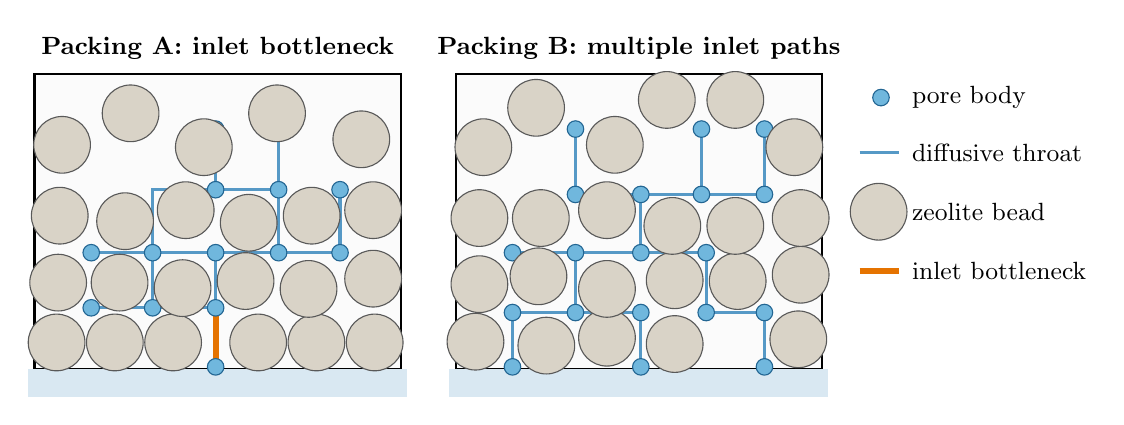
\begin{tikzpicture}[
 beadS/.style={circle,draw=black!65,fill=zeogray,minimum size=7.2mm,inner sep=0pt},
 beadM/.style={circle,draw=black!65,fill=zeogray,minimum size=7.2mm,inner sep=0pt},
 beadL/.style={circle,draw=black!65,fill=zeogray,minimum size=7.2mm,inner sep=0pt},
 pore/.style={circle,draw=co2blue!80!black,fill=poreblue,minimum size=2.1mm,inner sep=0pt},
 throat/.style={draw=co2blue!80,line width=1.15pt},
 bottleneck/.style={draw=orange!90!black,line width=2.2pt},
 paneltitle/.style={font=\small\bfseries,align=center},
 note/.style={font=\small,align=left}]

% Packing A: one restricted inlet-connected route.
\begin{scope}[shift={(0,0)}]
\fill[gray!3] (0,0) rectangle (4.65,3.75); \draw[thick] (0,0) rectangle (4.65,3.75);
\fill[co2blue!18] (-0.08,-0.35) rectangle (4.73,0);
\node[paneltitle] at (2.325,4.08) {Packing A: inlet bottleneck};
% The complete connected pore network is blue. It has no direct inlet
% connection except through the single orange bottleneck at x=2.30.
\draw[throat] (0.72,0.78)--(1.50,0.78)--(1.50,1.48)--(0.72,1.48);
\draw[throat] (1.50,0.78)--(2.30,0.78)--(2.30,1.48)--(1.50,1.48);
\draw[throat] (2.30,1.48)--(3.10,1.48)--(3.10,2.28)--(2.30,2.28)--(1.50,2.28)--(1.50,1.48);
\draw[throat] (3.10,1.48)--(3.88,1.48)--(3.88,2.28);
\draw[throat] (2.30,2.28)--(2.30,3.05); \draw[throat] (3.10,2.28)--(3.10,3.05);
% The only reservoir-to-network connection and its accessible backbone.
\draw[bottleneck] (2.30,0.03)--(2.30,0.78);
\draw[throat] (2.30,0.78)--(2.30,1.48)--(3.10,1.48)--(3.10,2.28)--(2.30,2.28)--(2.30,3.05);
\foreach \x/\y in {0.72/0.78,1.50/0.78,0.72/1.48,1.50/1.48,3.88/1.48,3.88/2.28,3.10/3.05} \node[pore] at (\x,\y) {};
\foreach \x/\y in {2.30/0.03,2.30/0.78,2.30/1.48,3.10/1.48,3.10/2.28,2.30/2.28,2.30/3.05} \node[pore] at (\x,\y) {};
% A nearly closed bottom layer: neighbouring beads touch/overlap visually, so
% no additional inlet opening can be inferred.
\node[beadM] at (0.28,0.34) {}; \node[beadM] at (1.02,0.34) {}; \node[beadM] at (1.76,0.34) {}; \node[beadM] at (2.84,0.34) {}; \node[beadM] at (3.58,0.34) {}; \node[beadM] at (4.32,0.34) {};
\node[beadM] at (0.30,1.10) {}; \node[beadM] at (1.08,1.10) {}; \node[beadM] at (1.88,1.03) {}; \node[beadM] at (2.68,1.12) {}; \node[beadM] at (3.48,1.02) {}; \node[beadM] at (4.30,1.15) {};
\node[beadM] at (0.32,1.95) {}; \node[beadM] at (1.15,1.88) {}; \node[beadM] at (1.92,2.02) {}; \node[beadM] at (2.72,1.86) {}; \node[beadM] at (3.52,1.95) {}; \node[beadM] at (4.30,2.02) {};
\node[beadM] at (0.35,2.85) {}; \node[beadM] at (1.22,3.25) {}; \node[beadM] at (2.15,2.82) {}; \node[beadM] at (3.08,3.25) {}; \node[beadM] at (4.15,2.92) {};
\end{scope}

% Packing B: several parallel inlet-connected routes.
\begin{scope}[shift={(5.35,0)}]
\fill[gray!3] (0,0) rectangle (4.65,3.75); \draw[thick] (0,0) rectangle (4.65,3.75);
\fill[co2blue!18] (-0.08,-0.35) rectangle (4.73,0);
\node[paneltitle] at (2.325,4.08) {Packing B: multiple inlet paths};
\draw[throat] (0.72,0.03)--(0.72,0.72)--(1.52,0.72)--(1.52,1.48)--(2.35,1.48)--(2.35,2.22)--(3.12,2.22)--(3.12,3.05);
\draw[throat] (2.35,0.03)--(2.35,0.72)--(1.52,0.72);
\draw[throat] (3.92,0.03)--(3.92,0.72)--(3.18,0.72)--(3.18,1.48)--(2.35,1.48);
\draw[throat] (0.72,1.48)--(1.52,1.48); \draw[throat] (2.35,2.22)--(1.52,2.22)--(1.52,3.05);
\draw[throat] (3.12,2.22)--(3.92,2.22)--(3.92,3.05);
\foreach \x/\y in {0.72/0.03,0.72/0.72,1.52/0.72,1.52/1.48,2.35/1.48,2.35/2.22,3.12/2.22,3.12/3.05,2.35/0.03,2.35/0.72,3.92/0.03,3.92/0.72,3.18/0.72,3.18/1.48,0.72/1.48,1.52/2.22,1.52/3.05,3.92/2.22,3.92/3.05} \node[pore] at (\x,\y) {};
\node[beadS] at (0.25,0.35) {}; \node[beadL] at (1.15,0.30) {}; \node[beadS] at (1.92,0.40) {}; \node[beadM] at (2.78,0.32) {}; \node[beadL] at (4.35,0.38) {};
\node[beadL] at (0.30,1.08) {}; \node[beadS] at (1.05,1.18) {}; \node[beadM] at (1.92,1.02) {}; \node[beadL] at (2.78,1.13) {}; \node[beadS] at (3.58,1.12) {}; \node[beadM] at (4.38,1.20) {};
\node[beadS] at (0.30,1.92) {}; \node[beadM] at (1.08,1.92) {}; \node[beadL] at (1.92,2.02) {}; \node[beadS] at (2.75,1.82) {}; \node[beadM] at (3.55,1.82) {}; \node[beadL] at (4.38,1.92) {};
\node[beadM] at (0.35,2.82) {}; \node[beadL] at (1.02,3.32) {}; \node[beadS] at (2.02,2.85) {}; \node[beadM] at (2.68,3.42) {}; \node[beadL] at (3.55,3.42) {}; \node[beadS] at (4.30,2.82) {};
\end{scope}

\node[pore] at (10.75,3.45) {}; \node[note,anchor=west] at (11.02,3.45) {pore body};
\draw[throat] (10.48,2.75)--(10.98,2.75); \node[note,anchor=west] at (11.02,2.75) {diffusive throat};
\node[beadM] at (10.72,2.0) {}; \node[note,anchor=west] at (11.02,2.0) {zeolite bead};
\draw[bottleneck] (10.48,1.25)--(10.98,1.25); \node[note,anchor=west] at (11.02,1.25) {inlet bottleneck};
\end{tikzpicture}%
}
\caption{Two illustrative monodisperse beds with different random arrangements.
Blue lines indicate the connected pore network. In Packing A, the closely
packed bottom layer leaves one narrow entrance (orange), so all transport must
first pass through this bottleneck. Packing B has several independent inlet
connections and parallel routes. The networks are schematic working hypotheses
to be tested.}
\label{fig:problem}
\end{figure}

\newpage
\section{Hypothesis and objectives}
The working hypothesis is:
\begin{quote}\setstretch{1.07}\itshape
Beds with similar porosity can have different transient uptake because their
inlet-connected void paths differ. A network-accessibility descriptor should
therefore predict effective transport better than porosity alone.
\end{quote}
This is a hypothesis, not a known result. The objectives are to:
\begin{enumerate}
\item quantify packing-to-packing variation under otherwise identical conditions;
\item build a conservative pore-network reference model for CO$_2$ diffusion and adsorption;
\item reduce every reference curve to one effective diffusivity in a 1D model; and
\item derive and test an interpretable closure from pore accessibility to effective diffusivity.
\end{enumerate}

\section{Proposed hybrid modelling framework}
\begin{figure}[!ht]
\centering
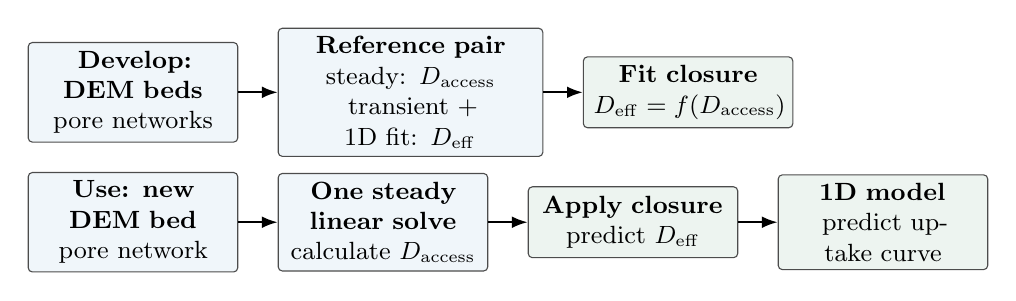
\begin{tikzpicture}[node distance=5mm and 5mm,
 box/.style={draw=black!70,rounded corners=1.5pt,minimum height=9mm,text width=2.45cm,align=center,font=\small,inner sep=3pt},
 physics/.style={box,fill=co2blue!7}, reduced/.style={box,fill=modelgreen!10},
 arr/.style={-{Latex[length=2mm]},thick}]
\node[physics] (train) {\textbf{Develop: DEM beds}\\pore networks};
\node[physics,right=of train,text width=3.15cm] (targets) {\textbf{Reference pair}\\steady: $D_{\mathrm{access}}$\\transient + 1D fit: $D_{\mathrm{eff}}$};
\node[reduced,right=of targets] (closure) {\textbf{Fit closure}\\$D_{\mathrm{eff}}=f(D_{\mathrm{access}})$};
\draw[arr] (train)--(targets); \draw[arr] (targets)--(closure);
\node[physics] (new) at (0,-1.65) {\textbf{Use: new DEM bed}\\pore network};
\node[physics,right=of new] (newacc) {\textbf{One steady linear solve}\\calculate $D_{\mathrm{access}}$};
\node[reduced,right=of newacc] (predict) {\textbf{Apply closure}\\predict $D_{\mathrm{eff}}$};
\node[reduced,right=of predict] (uptake) {\textbf{1D model}\\predict uptake curve};
\draw[arr] (new)--(newacc); \draw[arr] (newacc)--(predict); \draw[arr] (predict)--(uptake);
\end{tikzpicture}
\caption{Two separate stages. During development, detailed simulations provide
paired values of $D_{\mathrm{access}}$ and $D_{\mathrm{eff}}$ for fitting the
closure. For a new bed, the fitted closure supplies $D_{\mathrm{eff}}$ to the
fast 1D adsorption model; no transient pore-network simulation is required.}
\label{fig:workflow}
\end{figure}

\paragraph{WP1: Controlled packing ensemble.}
Generate independent cylindrical beds of identical zeolite beads by DEM. Keep
the particle number, bead size, tube size and operating conditions fixed; change
only the random insertion seed. Check settling, overlaps, bed height and local
and bulk porosity.

\paragraph{WP2: Structure-resolved reference model.}
Convert each void space into connected pore bodies and throats. Solve molecular
diffusion on this network and couple gas loss exactly to Langmuir equilibrium
and linear-driving-force uptake of the particles. Verify connectivity, void
volume, numerical convergence and total mass conservation.

\paragraph{WP3: Define the target and the structural predictor.}
For each bed, obtain the reference $D_{\mathrm{eff}}$ by first running the full
transient pore-network diffusion--adsorption model and then repeatedly solving
the 1D model while fitting its transport coefficient. Thus,
$D_{\mathrm{eff}}$ is the \emph{target bed-scale coefficient}. Separately,
impose a unit concentration difference between the inlet and an interior plane.
One steady linear network solve gives the conductance
$G_{\mathrm{access}}$ [m$^3$\,s$^{-1}$] and the structural descriptor
\[
D_{\mathrm{access}}=\frac{G_{\mathrm{access}}H}{A_{\mathrm{tube}}}.
\]
Here, $H$ is the bed height and $A_{\mathrm{tube}}$ is the tube cross-sectional
area. Unlike $D_{\mathrm{eff}}$, $D_{\mathrm{access}}$ needs no time integration,
adsorption calculation or parameter optimization. It is therefore much faster
and measures how easily the inlet is connected to the interior.

\paragraph{WP4: Closure and predictive test.}
Develop and compare three mappings for the same target, $D_{\mathrm{eff}}$:
\[
\text{porosity: }D_{\mathrm{eff}}=a_0+a_1\varepsilon_b,\qquad
\text{proportional: }D_{\mathrm{eff}}=\alpha D_{\mathrm{access}},\qquad
\text{power law: }\frac{D_{\mathrm{eff}}}{D_m}
=C\left(\frac{D_{\mathrm{access}}}{D_m}\right)^n .
\]
Here, $\varepsilon_b$ is bed porosity, $D_m$ is molecular diffusivity, and the
coefficients are learned from the training beds. Leave complete beds out during
fitting, predict their $D_{\mathrm{eff}}$, and use that value in the 1D model to
predict their uptake curves. Repeat the accessibility calculation at several
interior depths to check that the comparison does not depend on one selected
plane.

\section{Expected outcome, scope and success criterion}
For a new packing, one steady accessibility solve will provide
$D_{\mathrm{access}}$; the selected closure will predict $D_{\mathrm{eff}}$;
and the 1D model will return the transient mean CO$_2$ loading. This replaces
the transient pore-network calculation while retaining a link to structure.
The first study isolates isothermal diffusion in stagnant gas; pressure drop,
forced-flow breakthrough, heat effects and mixtures remain outside its scope.
The concept succeeds if the reference model is conservative, the 1D reduction
is accurate, and accessibility predicts withheld beds better than porosity. If
not, the proposed structure-based closure is not justified. Either outcome
provides a clear modelling decision.

\end{document}
